\tikzset{>=latex} % for LaTeX arrow head
\colorlet{Bcol}{violet!90}
\colorlet{BFcol}{red!60!black}
\colorlet{veccol}{green!45!black}
\colorlet{Icol}{blue!70!black}
\tikzstyle{BField}=[->,thick,Bcol]
\tikzstyle{current}=[->,Icol] %thick,
\tikzstyle{force}=[->,thick,BFcol]
\tikzstyle{vector}=[->,thick,veccol]
\tikzstyle{velocity}=[->,very thick,vcol]
\tikzstyle{charge+}=[very thin,draw=black,top color=red!50,bottom color=red!90!black,shading angle=20,circle,inner sep=0.5]
\tikzstyle{charge-}=[very thin,draw=black,top color=blue!50,bottom color=blue!80,shading angle=20,circle,inner sep=0.5]
\tikzstyle{metal}=[top color=black!15,bottom color=black!25,middle color=black!5,shading angle=10]
\tikzset{
  BFieldLine/.style={thick,Bcol,decoration={markings,mark=at position #1 with {\arrow{latex}}},
                                 postaction={decorate}},
  BFieldLine/.default=0.5,
  pics/Bin/.style={
    code={
      \def\R{0.12}
      \draw[pic actions,line width=0.6,#1] % ,thick
        (0,0) circle (\R) (-135:.75*\R) -- (45:.75*\R) (-45:.75*\R) -- (135:.75*\R);
  }},
  pics/Bout/.style={
    code={
      \def\R{0.12}
      \draw[pic actions,line width=0.6,#1,fill=white] (0,0) circle (\R);
      \fill[pic actions,#1] (0,0) circle (0.3*\R);
  }},
  pics/Bin/.default=Bcol,
  pics/Bout/.default=Bcol,
}

% CURRENT IN B FIELD




% B FIELD perpendicular to square circuit 2D


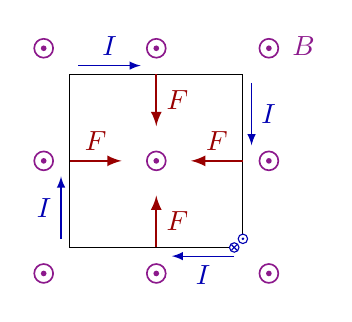
\begin{tikzpicture}
  \def\H{2.2}
  \def\W{2.2}
  \def\NB{3}
  
  % ELECTRIC FIELD
  \foreach \i [evaluate={\y=-0.15*\W+(\i-1)*1.3*\H/(\NB-1);}] in {1,...,\NB}{
    \foreach \j [evaluate={\x=-0.15*\W+(\j-1)*1.3*\W/(\NB-1);}] in {1,...,\NB}{
      \pic at (\x,\y) {Bout};
    }
  }
  \node[Bcol] at (1.35*\W,1.16*\W) {$\vb{B}$};
  
  % CIRCUIT
  \draw (0,0) rectangle (\W,\H);
  \draw[current] ( 0.05*\W, 1.05*\H) --++ ( 0.36*\W,0) node[midway,above] {$I$};
  \draw[current] ( 0.95*\W,-0.05*\H) --++ (-0.36*\W,0) node[midway,below] {$I$};
  \draw[current] ( 1.05*\W, 0.95*\H) --++ (0,-0.36*\H) node[midway,right] {$I$};
  \draw[current] (-0.05*\W, 0.05*\H) --++ (0, 0.36*\H) node[midway,left] {$I$};
  \fill[white] (\W,0) circle (0.06);
  %\fill (\W,0.03*\W) circle (0.04);
  %\fill (0.97*\W,0) circle (0.04);
  \pic[scale=0.5] at (0.95*\W,0) {Bin={Icol,fill=white,line width=0.4}};
  \pic[scale=0.5] at (\W,0.05*\H) {Bout={Icol,line width=0.4}};
  
  % FORCE
  \draw[force] (\W/2,\H) --++ (0,-0.3*\H) node[force,midway,right] {$\vb{F}$};
  \draw[force] (\W/2, 0) --++ (0, 0.3*\H) node[force,midway,right] {$\vb{F}$};
  \draw[force] (\W,\H/2) --++ (-0.3*\W,0) node[force,midway,above] {$\vb{F}$};
  \draw[force] ( 0,\H/2) --++ ( 0.3*\W,0) node[force,midway,above] {$\vb{F}$};
  
\end{tikzpicture}
